\documentclass{article}
\usepackage{amsmath}
\usepackage{amsfonts}
\usepackage{amssymb}
\usepackage{graphicx}
\usepackage{hyperref}
\usepackage{xcolor}
\usepackage{listings}
\usepackage[left=1.3cm, right=1.3cm, top=0.6in, bottom=0.9in]{geometry}
%-------------------------------------------
\newtheorem{theorem}{Theorem}
\newtheorem{acknowledgement}[theorem]{Acknowledgement}
\newtheorem{algorithm}[theorem]{Algorithm}
\newtheorem{axiom}[theorem]{Axiom}
\newtheorem{case}[theorem]{Case}
\newtheorem{claim}[theorem]{Claim}
\newtheorem{conclusion}[theorem]{Conclusion}
\newtheorem{condition}[theorem]{Condition}
\newtheorem{conjecture}[theorem]{Conjecture}
\newtheorem{corollary}[theorem]{Corollary}
\newtheorem{criterion}[theorem]{Criterion}
\newtheorem{definition}[theorem]{Definition}
\newtheorem{example}[theorem]{Example}
\newtheorem{exercise}[theorem]{Exercise}
\newtheorem{lemma}[theorem]{Lemma}
\newtheorem{notation}[theorem]{Notation}
\newtheorem{problem}[theorem]{Problem}
\newtheorem{proposition}[theorem]{Proposition}
\newtheorem{remark}[theorem]{Remark}
\newtheorem{solution}[theorem]{Solution}
\newtheorem{summary}[theorem]{Summary}
\newenvironment{proof}[1][Proof]{\textbf{#1.} }{\ \rule{0.5em}{0.5em}}
\setlength{\parindent}{0.3in}

\lstdefinestyle{python}{
  language=Python,
  basicstyle=\ttfamily\small,
  keywordstyle=\color{blue},
  stringstyle=\color{red},
  commentstyle=\color{gray},
  identifierstyle=\color{black},
  showstringspaces=false,
  breaklines=true,
  columns=fullflexible,
  frame=single
}

\begin{document}

\begin{flushright}
\textbf{Jaskirat Singh Maskeen, 23110146 \\
4 February, 2026\\
{\color{blue}\href{https://github.com/jsmaskeen/CS431-Assignments/tree/assn4}{GitHub Repository}}\\ 
CTF Username: \texttt{23110146}}
\end{flushright}

\begin{center}
\textbf{CS 431: Computer and Network Security  \\
Assignment 4} \\
\end{center}

\noindent
\subsubsection*{InsIIT | \texttt{python3 solution.py 1}}
{Flag} : \texttt{cns431\{you\_snoopy\_doo\_didnt\_i\_tell\_you\_to\_get\_off\_my\_lawn\}}\\ (Note: while copying the flag, underscores are not copied. Some latex issue)\\ 
We check the \texttt{/robots.txt} file, and find a disallowed path (\texttt{/fade/to/black}), which led to the flag. 

\subsubsection*{oreo | \texttt{python3 solution.py 2}}
{Flag} : \texttt{ican\{1ick\_twi5t\_dunk\}}\\  (Note: while copying the flag, underscores are not copied. Some latex issue)\\ 
The challenge name and text on the webpage hints at using some cookies. We observe the cookies (first, using the extension, \href{https://www.editthiscookie.com/}{Edit This Cookie}, later using Cookie object in requests module.) The server used base64-encoded cookies. We notice that the flavor is set to, `strawberry'. We change it to `chocolate' (base 64 encoded). Refreshing the page, gives us the flag.

\subsubsection*{events | \texttt{python3 solution.py 3}}
{Flag} : \texttt{br@V0---\{yoU\_F0und\_m3\}}\\  (Note: while copying the flag, underscores are not copied. Some latex issue)\\ 
The flag was hidden in a CSS file as a comment. By fetching the file and extracting the comment, the flag was obtained.

\subsubsection*{CNSxSS | \texttt{python3 solution.py 4}}
{Flag} : \texttt{cns431\_d4ng3r\_n0\_val1dat1on\_xss}\\ (Note: while copying the flag, underscores are not copied. Some latex issue)\\ 
We observed that, we can get arbitrary Javascript injection, by passing in \texttt{"; arbitrary\_javascript; //}. We make a small webhook using \href{https://webhook.site/}{https://webhook.site/}, then send a payload which creates a new image, with source being `webhook.site/blahblah?k=blah'. Then we send this to overlords. When the overlords open the page, the code tries to get the url specified, and we can see the exact request at \href{https://webhook.site/}{https://webhook.site/} interface. We see the request's headers, and we get the flag.\\
\vspace{10pt}
\noindent
\begin{minipage}[t]{0.49\textwidth}
\vspace{0pt}
\centering
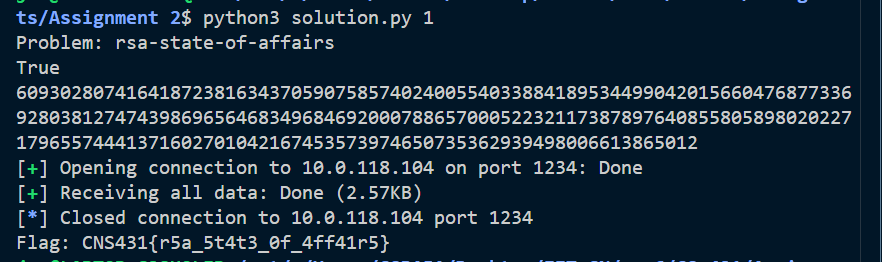
\includegraphics[width=\linewidth]{../images/1.png}
% \vspace{0.5cm}
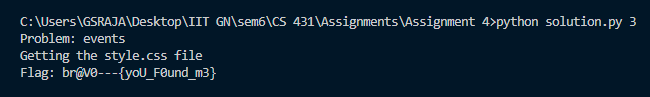
\includegraphics[width=\linewidth]{../images/3.png}
\end{minipage}
\hfill
\begin{minipage}[t]{0.49\textwidth}
\vspace{0pt}
\centering
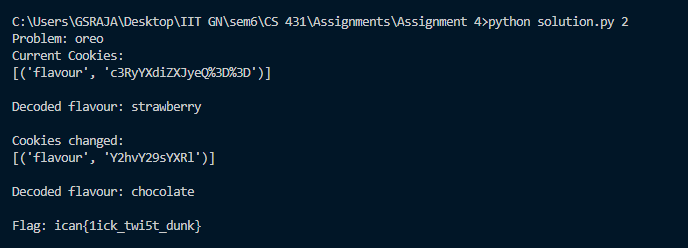
\includegraphics[width=\linewidth]{../images/2.png}
% \vspace{0.5cm}
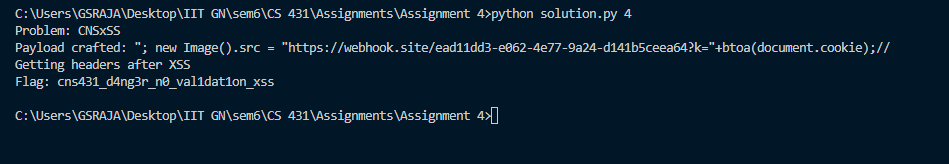
\includegraphics[width=\linewidth]{../images/4.png}
\end{minipage}

\newpage
\section*{Source Code: solution.py}
\lstset{style=python}
\lstinputlisting{./../solution.py}
\end{document}